\documentclass[1p]{elsarticle_modified}
%\bibliographystyle{elsarticle-num}

%\usepackage[colorlinks]{hyperref}
%\usepackage{abbrmath_seonhwa} %\Abb, \Ascr, \Acal ,\Abf, \Afrak
\usepackage{amsfonts}
\usepackage{amssymb}
\usepackage{amsmath}
\usepackage{amsthm}
\usepackage{scalefnt}
\usepackage{amsbsy}
\usepackage{kotex}
\usepackage{caption}
\usepackage{subfig}
\usepackage{color}
\usepackage{graphicx}
\usepackage{xcolor} %% white, black, red, green, blue, cyan, magenta, yellow
\usepackage{float}
\usepackage{setspace}
\usepackage{hyperref}

\usepackage{tikz}
\usetikzlibrary{arrows}

\usepackage{multirow}
\usepackage{array} % fixed length table
\usepackage{hhline}

%%%%%%%%%%%%%%%%%%%%%
\makeatletter
\renewcommand*\env@matrix[1][\arraystretch]{%
	\edef\arraystretch{#1}%
	\hskip -\arraycolsep
	\let\@ifnextchar\new@ifnextchar
	\array{*\c@MaxMatrixCols c}}
\makeatother %https://tex.stackexchange.com/questions/14071/how-can-i-increase-the-line-spacing-in-a-matrix
%%%%%%%%%%%%%%%

\usepackage[normalem]{ulem}

\newcommand{\msout}[1]{\ifmmode\text{\sout{\ensuremath{#1}}}\else\sout{#1}\fi}
%SOURCE: \msout is \stkout macro in https://tex.stackexchange.com/questions/20609/strikeout-in-math-mode

\newcommand{\cancel}[1]{
	\ifmmode
	{\color{red}\msout{#1}}
	\else
	{\color{red}\sout{#1}}
	\fi
}

\newcommand{\add}[1]{
	{\color{blue}\uwave{#1}}
}

\newcommand{\replace}[2]{
	\ifmmode
	{\color{red}\msout{#1}}{\color{blue}\uwave{#2}}
	\else
	{\color{red}\sout{#1}}{\color{blue}\uwave{#2}}
	\fi
}

\newcommand{\Sol}{\mathcal{S}} %segment
\newcommand{\D}{D} %diagram
\newcommand{\A}{\mathcal{A}} %arc


%%%%%%%%%%%%%%%%%%%%%%%%%%%%%5 test

\def\sl{\operatorname{\textup{SL}}(2,\Cbb)}
\def\psl{\operatorname{\textup{PSL}}(2,\Cbb)}
\def\quan{\mkern 1mu \triangleright \mkern 1mu}

\theoremstyle{definition}
\newtheorem{thm}{Theorem}[section]
\newtheorem{prop}[thm]{Proposition}
\newtheorem{lem}[thm]{Lemma}
\newtheorem{ques}[thm]{Question}
\newtheorem{cor}[thm]{Corollary}
\newtheorem{defn}[thm]{Definition}
\newtheorem{exam}[thm]{Example}
\newtheorem{rmk}[thm]{Remark}
\newtheorem{alg}[thm]{Algorithm}

\newcommand{\I}{\sqrt{-1}}
\begin{document}

%\begin{frontmatter}
%
%\title{Boundary parabolic representations of knots up to 8 crossings}
%
%%% Group authors per affiliation:
%\author{Yunhi Cho} 
%\address{Department of Mathematics, University of Seoul, Seoul, Korea}
%\ead{yhcho@uos.ac.kr}
%
%
%\author{Seonhwa Kim} %\fnref{s_kim}}
%\address{Center for Geometry and Physics, Institute for Basic Science, Pohang, 37673, Korea}
%\ead{ryeona17@ibs.re.kr}
%
%\author{Hyuk Kim}
%\address{Department of Mathematical Sciences, Seoul National University, Seoul 08826, Korea}
%\ead{hyukkim@snu.ac.kr}
%
%\author{Seokbeom Yoon}
%\address{Department of Mathematical Sciences, Seoul National University, Seoul, 08826,  Korea}
%\ead{sbyoon15@snu.ac.kr}
%
%\begin{abstract}
%We find all boundary parabolic representation of knots up to 8 crossings.
%
%\end{abstract}
%\begin{keyword}
%    \MSC[2010] 57M25 
%\end{keyword}
%
%\end{frontmatter}

%\linenumbers
%\tableofcontents
%
\newcommand\colored[1]{\textcolor{white}{\rule[-0.35ex]{0.8em}{1.4ex}}\kern-0.8em\color{red} #1}%
%\newcommand\colored[1]{\textcolor{white}{ #1}\kern-2.17ex	\textcolor{white}{ #1}\kern-1.81ex	\textcolor{white}{ #1}\kern-2.15ex\color{red}#1	}

{\Large $\underline{12n_{0087}~(K12n_{0087})}$}

\setlength{\tabcolsep}{10pt}
\renewcommand{\arraystretch}{1.6}
\vspace{1cm}\begin{tabular}{m{100pt}>{\centering\arraybackslash}m{274pt}}
\multirow{5}{120pt}{
	\centering
	\includegraphics[width=112pt]{../../../GIT/diagram.site/Diagrams/png/2176_12n_0087.png}\\
\ \ \ A knot diagram\footnotemark}&
\allowdisplaybreaks
\textbf{Linearized knot diagam} \\
\cline{2-2}
 &
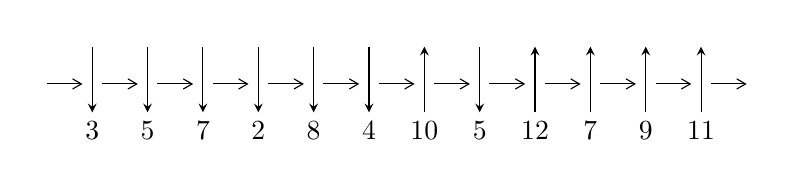
\begin{tikzpicture}[x=20pt, y=17pt]
	% nodes
	\node (C0) at (0, 0) {};
	\node (C1) at (1, 0) {};
	\node (C1U) at (1, +1) {};
	\node (C1D) at (1, -1) {3};

	\node (C2) at (2, 0) {};
	\node (C2U) at (2, +1) {};
	\node (C2D) at (2, -1) {5};

	\node (C3) at (3, 0) {};
	\node (C3U) at (3, +1) {};
	\node (C3D) at (3, -1) {7};

	\node (C4) at (4, 0) {};
	\node (C4U) at (4, +1) {};
	\node (C4D) at (4, -1) {2};

	\node (C5) at (5, 0) {};
	\node (C5U) at (5, +1) {};
	\node (C5D) at (5, -1) {8};

	\node (C6) at (6, 0) {};
	\node (C6U) at (6, +1) {};
	\node (C6D) at (6, -1) {4};

	\node (C7) at (7, 0) {};
	\node (C7U) at (7, +1) {};
	\node (C7D) at (7, -1) {10};

	\node (C8) at (8, 0) {};
	\node (C8U) at (8, +1) {};
	\node (C8D) at (8, -1) {5};

	\node (C9) at (9, 0) {};
	\node (C9U) at (9, +1) {};
	\node (C9D) at (9, -1) {12};

	\node (C10) at (10, 0) {};
	\node (C10U) at (10, +1) {};
	\node (C10D) at (10, -1) {7};

	\node (C11) at (11, 0) {};
	\node (C11U) at (11, +1) {};
	\node (C11D) at (11, -1) {9};

	\node (C12) at (12, 0) {};
	\node (C12U) at (12, +1) {};
	\node (C12D) at (12, -1) {11};
	\node (C13) at (13, 0) {};

	% arrows
	\draw[->,>={angle 60}]
	(C0) edge (C1) (C1) edge (C2) (C2) edge (C3) (C3) edge (C4) (C4) edge (C5) (C5) edge (C6) (C6) edge (C7) (C7) edge (C8) (C8) edge (C9) (C9) edge (C10) (C10) edge (C11) (C11) edge (C12) (C12) edge (C13) ;	\draw[->,>=stealth]
	(C1U) edge (C1D) (C2U) edge (C2D) (C3U) edge (C3D) (C4U) edge (C4D) (C5U) edge (C5D) (C6U) edge (C6D) (C7D) edge (C7U) (C8U) edge (C8D) (C9D) edge (C9U) (C10D) edge (C10U) (C11D) edge (C11U) (C12D) edge (C12U) ;
	\end{tikzpicture} \\
\hhline{~~} \\& 
\textbf{Solving Sequence} \\ \cline{2-2} 
 &
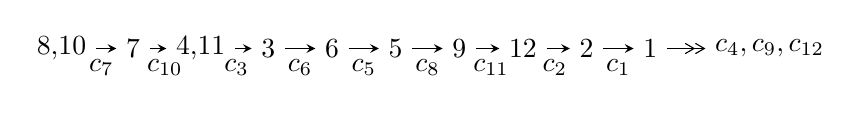
\begin{tikzpicture}[x=23pt, y=7pt]
	% node
	\node (A0) at (-1/8, 0) {8,10};
	\node (A1) at (1, 0) {7};
	\node (A2) at (33/16, 0) {4,11};
	\node (A3) at (25/8, 0) {3};
	\node (A4) at (33/8, 0) {6};
	\node (A5) at (41/8, 0) {5};
	\node (A6) at (49/8, 0) {9};
	\node (A7) at (57/8, 0) {12};
	\node (A8) at (65/8, 0) {2};
	\node (A9) at (73/8, 0) {1};
	\node (C1) at (1/2, -1) {$c_{7}$};
	\node (C2) at (3/2, -1) {$c_{10}$};
	\node (C3) at (21/8, -1) {$c_{3}$};
	\node (C4) at (29/8, -1) {$c_{6}$};
	\node (C5) at (37/8, -1) {$c_{5}$};
	\node (C6) at (45/8, -1) {$c_{8}$};
	\node (C7) at (53/8, -1) {$c_{11}$};
	\node (C8) at (61/8, -1) {$c_{2}$};
	\node (C9) at (69/8, -1) {$c_{1}$};
	\node (A10) at (11, 0) {$c_{4},c_{9},c_{12}$};

	% edge
	\draw[->,>=stealth]	
	(A0) edge (A1) (A1) edge (A2) (A2) edge (A3) (A3) edge (A4) (A4) edge (A5) (A5) edge (A6) (A6) edge (A7) (A7) edge (A8) (A8) edge (A9) ;
	\draw[->>,>={angle 60}]	
	(A9) edge (A10);
\end{tikzpicture} \\ 

\end{tabular} \\

\footnotetext{
The image of knot diagram is generated by the software ``\textbf{Draw programme}" developed by Andrew Bartholomew(\url{http://www.layer8.co.uk/maths/draw/index.htm\#Running-draw}), where we modified some parts for our purpose(\url{https://github.com/CATsTAILs/LinksPainter}).
}\phantom \\ \newline 
\centering \textbf{Ideals for irreducible components\footnotemark of $X_{\text{par}}$} 
 
\begin{align*}
I^u_{1}&=\langle 
2.21397\times10^{102} u^{43}-1.21296\times10^{103} u^{42}+\cdots+5.90528\times10^{102} b-1.68663\times10^{103},\\
\phantom{I^u_{1}}&\phantom{= \langle  }2.74407\times10^{102} u^{43}-1.57666\times10^{103} u^{42}+\cdots+2.95264\times10^{102} a-2.53471\times10^{103},\;u^{44}-5 u^{43}+\cdots+16 u-4\rangle \\
I^u_{2}&=\langle 
u^8-2 u^7+3 u^6-3 u^5+4 u^4-4 u^3+3 u^2+b-2 u+1,\\
\phantom{I^u_{2}}&\phantom{= \langle  }3 u^8-4 u^7+8 u^6-7 u^5+13 u^4-9 u^3+11 u^2+a-6 u+6,\;u^9- u^8+2 u^7- u^6+3 u^5- u^4+2 u^3+u+1\rangle \\
I^u_{3}&=\langle 
-3 u^2 a+4 a u+u^2+5 b+3 a+7 u+4,\;-2 u^2 a+a^2- a u+12 u^2- a+5 u+22,\;u^3+u^2+2 u+1\rangle \\
I^u_{4}&=\langle 
b- u,\;a,\;u^3+u^2+2 u+1\rangle \\
\\
I^v_{1}&=\langle 
a,\;3 b+v-5,\;v^2-7 v+1\rangle \\
\end{align*}
\raggedright * 5 irreducible components of $\dim_{\mathbb{C}}=0$, with total 64 representations.\\
\footnotetext{All coefficients of polynomials are rational numbers. But the coefficients are sometimes approximated in decimal forms when there is not enough margin.}
\newpage
\renewcommand{\arraystretch}{1}
\centering \section*{I. $I^u_{1}= \langle 2.21\times10^{102} u^{43}-1.21\times10^{103} u^{42}+\cdots+5.91\times10^{102} b-1.69\times10^{103},\;2.74\times10^{102} u^{43}-1.58\times10^{103} u^{42}+\cdots+2.95\times10^{102} a-2.53\times10^{103},\;u^{44}-5 u^{43}+\cdots+16 u-4 \rangle$}
\flushleft \textbf{(i) Arc colorings}\\
\begin{tabular}{m{7pt} m{180pt} m{7pt} m{180pt} }
\flushright $a_{8}=$&$\begin{pmatrix}1\\0\end{pmatrix}$ \\
\flushright $a_{10}=$&$\begin{pmatrix}0\\u\end{pmatrix}$ \\
\flushright $a_{7}=$&$\begin{pmatrix}1\\u^2\end{pmatrix}$ \\
\flushright $a_{4}=$&$\begin{pmatrix}-0.929363 u^{43}+5.33983 u^{42}+\cdots-18.7982 u+8.58457\\-0.374913 u^{43}+2.05402 u^{42}+\cdots-21.5523 u+2.85613\end{pmatrix}$ \\
\flushright $a_{11}=$&$\begin{pmatrix}u\\u^3+u\end{pmatrix}$ \\
\flushright $a_{3}=$&$\begin{pmatrix}-1.07481 u^{43}+6.05592 u^{42}+\cdots-25.5449 u+8.66865\\-0.409892 u^{43}+2.21633 u^{42}+\cdots-21.9557 u+2.81153\end{pmatrix}$ \\
\flushright $a_{6}=$&$\begin{pmatrix}0.145102 u^{43}-0.707901 u^{42}+\cdots+19.1582 u+1.02362\\0.147085 u^{43}-0.785533 u^{42}+\cdots+9.81828 u-1.73382\end{pmatrix}$ \\
\flushright $a_{5}=$&$\begin{pmatrix}0.292188 u^{43}-1.49343 u^{42}+\cdots+28.9765 u-0.710207\\0.147085 u^{43}-0.785533 u^{42}+\cdots+9.81828 u-1.73382\end{pmatrix}$ \\
\flushright $a_{9}=$&$\begin{pmatrix}-0.115004 u^{43}+0.603443 u^{42}+\cdots-8.54799 u+1.54989\\-0.253152 u^{43}+1.35100 u^{42}+\cdots-24.4831 u+3.51231\end{pmatrix}$ \\
\flushright $a_{12}=$&$\begin{pmatrix}-0.143897 u^{43}+0.773429 u^{42}+\cdots-15.0203 u+1.84872\\-0.289178 u^{43}+1.53362 u^{42}+\cdots-25.0070 u+3.61440\end{pmatrix}$ \\
\flushright $a_{2}=$&$\begin{pmatrix}-1.09992 u^{43}+6.16075 u^{42}+\cdots-35.4851 u+8.06492\\-0.238125 u^{43}+1.32996 u^{42}+\cdots-6.84876 u+1.04083\end{pmatrix}$ \\
\flushright $a_{1}=$&$\begin{pmatrix}0.138148 u^{43}-0.747554 u^{42}+\cdots+15.9351 u-1.96242\\0.280915 u^{43}-1.49627 u^{42}+\cdots+25.9447 u-3.73957\end{pmatrix}$\\&\end{tabular}
\flushleft \textbf{(ii) Obstruction class $= -1$}\\~\\
\flushleft \textbf{(iii) Cusp Shapes $= 25.5545 u^{43}-140.944 u^{42}+\cdots+1055.90 u-191.724$}\\~\\
\newpage\renewcommand{\arraystretch}{1}
\flushleft \textbf{(iv) u-Polynomials at the component}\newline \\
\begin{tabular}{m{50pt}|m{274pt}}
Crossings & \hspace{64pt}u-Polynomials at each crossing \\
\hline $$\begin{aligned}c_{1}\end{aligned}$$&$\begin{aligned}
&u^{44}+6 u^{43}+\cdots+29830 u+1
\end{aligned}$\\
\hline $$\begin{aligned}c_{2},c_{4}\end{aligned}$$&$\begin{aligned}
&u^{44}-14 u^{43}+\cdots-166 u-1
\end{aligned}$\\
\hline $$\begin{aligned}c_{3},c_{6}\end{aligned}$$&$\begin{aligned}
&u^{44}-5 u^{43}+\cdots+3072 u+512
\end{aligned}$\\
\hline $$\begin{aligned}c_{5},c_{8}\end{aligned}$$&$\begin{aligned}
&u^{44}-3 u^{43}+\cdots+4096 u-512
\end{aligned}$\\
\hline $$\begin{aligned}c_{7},c_{10}\end{aligned}$$&$\begin{aligned}
&u^{44}+5 u^{43}+\cdots-16 u-4
\end{aligned}$\\
\hline $$\begin{aligned}c_{9},c_{11}\end{aligned}$$&$\begin{aligned}
&u^{44}+7 u^{43}+\cdots+83 u-1
\end{aligned}$\\
\hline $$\begin{aligned}c_{12}\end{aligned}$$&$\begin{aligned}
&u^{44}-33 u^{43}+\cdots-6317 u+1
\end{aligned}$\\
\hline
\end{tabular}\\~\\
\newpage\renewcommand{\arraystretch}{1}
\flushleft \textbf{(v) Riley Polynomials at the component}\newline \\
\begin{tabular}{m{50pt}|m{274pt}}
Crossings & \hspace{64pt}Riley Polynomials at each crossing \\
\hline $$\begin{aligned}c_{1}\end{aligned}$$&$\begin{aligned}
&y^{44}+78 y^{43}+\cdots-889350874 y+1
\end{aligned}$\\
\hline $$\begin{aligned}c_{2},c_{4}\end{aligned}$$&$\begin{aligned}
&y^{44}-6 y^{43}+\cdots-29830 y+1
\end{aligned}$\\
\hline $$\begin{aligned}c_{3},c_{6}\end{aligned}$$&$\begin{aligned}
&y^{44}+63 y^{43}+\cdots-69206016 y+262144
\end{aligned}$\\
\hline $$\begin{aligned}c_{5},c_{8}\end{aligned}$$&$\begin{aligned}
&y^{44}+49 y^{43}+\cdots-15859712 y+262144
\end{aligned}$\\
\hline $$\begin{aligned}c_{7},c_{10}\end{aligned}$$&$\begin{aligned}
&y^{44}-3 y^{43}+\cdots-1304 y+16
\end{aligned}$\\
\hline $$\begin{aligned}c_{9},c_{11}\end{aligned}$$&$\begin{aligned}
&y^{44}-33 y^{43}+\cdots-6317 y+1
\end{aligned}$\\
\hline $$\begin{aligned}c_{12}\end{aligned}$$&$\begin{aligned}
&y^{44}-37 y^{43}+\cdots-39734481 y+1
\end{aligned}$\\
\hline
\end{tabular}\\~\\
\newpage\flushleft \textbf{(vi) Complex Volumes and Cusp Shapes}
$$\begin{array}{c|c|c}  
\text{Solutions to }I^u_{1}& \I (\text{vol} + \sqrt{-1}CS) & \text{Cusp shape}\\
 \hline 
\begin{aligned}
u &= \phantom{-}0.048281 + 1.061060 I \\
a &= \phantom{-}0.370251 + 0.083303 I \\
b &= -0.623557 - 0.693283 I\end{aligned}
 & -2.03545 - 1.53423 I & -2.00000 + 3.28440 I \\ \hline\begin{aligned}
u &= \phantom{-}0.048281 - 1.061060 I \\
a &= \phantom{-}0.370251 - 0.083303 I \\
b &= -0.623557 + 0.693283 I\end{aligned}
 & -2.03545 + 1.53423 I & -2.00000 - 3.28440 I \\ \hline\begin{aligned}
u &= -0.444024 + 0.972451 I \\
a &= -0.213577 - 0.298798 I \\
b &= -0.151321 - 0.361837 I\end{aligned}
 & -0.22354 - 3.19884 I & \phantom{-0.000000 -}0. + 5.55216 I \\ \hline\begin{aligned}
u &= -0.444024 - 0.972451 I \\
a &= -0.213577 + 0.298798 I \\
b &= -0.151321 + 0.361837 I\end{aligned}
 & -0.22354 + 3.19884 I & \phantom{-0.000000 } 0. - 5.55216 I \\ \hline\begin{aligned}
u &= \phantom{-}0.874663 + 0.275257 I \\
a &= \phantom{-}1.04774 + 1.16816 I \\
b &= \phantom{-}0.236448 + 0.150247 I\end{aligned}
 & \phantom{-}3.87014 - 2.97279 I & \phantom{-}3.60919 + 6.63471 I \\ \hline\begin{aligned}
u &= \phantom{-}0.874663 - 0.275257 I \\
a &= \phantom{-}1.04774 - 1.16816 I \\
b &= \phantom{-}0.236448 - 0.150247 I\end{aligned}
 & \phantom{-}3.87014 + 2.97279 I & \phantom{-}3.60919 - 6.63471 I \\ \hline\begin{aligned}
u &= \phantom{-}0.310742 + 1.065360 I \\
a &= \phantom{-}0.269693 + 1.146740 I \\
b &= -0.465484 + 0.146095 I\end{aligned}
 & \phantom{-}5.03100 + 0.55063 I & \phantom{-}1.92030 - 1.63801 I \\ \hline\begin{aligned}
u &= \phantom{-}0.310742 - 1.065360 I \\
a &= \phantom{-}0.269693 - 1.146740 I \\
b &= -0.465484 - 0.146095 I\end{aligned}
 & \phantom{-}5.03100 - 0.55063 I & \phantom{-}1.92030 + 1.63801 I \\ \hline\begin{aligned}
u &= \phantom{-}0.627914 + 0.971697 I \\
a &= -0.330748 - 0.066410 I \\
b &= -0.034558 + 0.334761 I\end{aligned}
 & \phantom{-}2.13500 + 7.76603 I & \phantom{-0.000000 } 0. - 12.26438 I \\ \hline\begin{aligned}
u &= \phantom{-}0.627914 - 0.971697 I \\
a &= -0.330748 + 0.066410 I \\
b &= -0.034558 - 0.334761 I\end{aligned}
 & \phantom{-}2.13500 - 7.76603 I & \phantom{-0.000000 -}0. + 12.26438 I\\
 \hline 
 \end{array}$$\newpage$$\begin{array}{c|c|c}  
\text{Solutions to }I^u_{1}& \I (\text{vol} + \sqrt{-1}CS) & \text{Cusp shape}\\
 \hline 
\begin{aligned}
u &= -1.088600 + 0.454876 I \\
a &= \phantom{-}0.415899 - 0.644451 I \\
b &= \phantom{-}0.653494 - 0.268396 I\end{aligned}
 & \phantom{-}2.35471 - 1.62269 I & \phantom{-0.000000 -}0. + 2.86308 I \\ \hline\begin{aligned}
u &= -1.088600 - 0.454876 I \\
a &= \phantom{-}0.415899 + 0.644451 I \\
b &= \phantom{-}0.653494 + 0.268396 I\end{aligned}
 & \phantom{-}2.35471 + 1.62269 I & \phantom{-0.000000 } 0. - 2.86308 I \\ \hline\begin{aligned}
u &= \phantom{-}1.171290 + 0.197003 I \\
a &= \phantom{-}0.058277 + 0.836682 I \\
b &= -1.49981 - 0.37516 I\end{aligned}
 & \phantom{-}4.40564 + 2.10618 I & \phantom{-0.000000 } 0 \\ \hline\begin{aligned}
u &= \phantom{-}1.171290 - 0.197003 I \\
a &= \phantom{-}0.058277 - 0.836682 I \\
b &= -1.49981 + 0.37516 I\end{aligned}
 & \phantom{-}4.40564 - 2.10618 I & \phantom{-0.000000 } 0 \\ \hline\begin{aligned}
u &= -0.625793 + 1.141240 I \\
a &= \phantom{-}0.475335 - 0.251871 I \\
b &= -1.43711 + 0.62601 I\end{aligned}
 & -0.60424 - 3.28908 I & \phantom{-0.000000 } 0 \\ \hline\begin{aligned}
u &= -0.625793 - 1.141240 I \\
a &= \phantom{-}0.475335 + 0.251871 I \\
b &= -1.43711 - 0.62601 I\end{aligned}
 & -0.60424 + 3.28908 I & \phantom{-0.000000 } 0 \\ \hline\begin{aligned}
u &= -0.231224 + 1.281260 I \\
a &= \phantom{-}2.55356 - 0.49814 I \\
b &= -3.85023 - 0.67062 I\end{aligned}
 & -4.23715 - 2.76938 I & -48.8073 + 0. I\phantom{ +0.000000I} \\ \hline\begin{aligned}
u &= -0.231224 - 1.281260 I \\
a &= \phantom{-}2.55356 + 0.49814 I \\
b &= -3.85023 + 0.67062 I\end{aligned}
 & -4.23715 + 2.76938 I & -48.8073 + 0. I\phantom{ +0.000000I} \\ \hline\begin{aligned}
u &= -1.271420 + 0.302065 I \\
a &= -0.143630 + 1.274350 I \\
b &= \phantom{-}0.295378 - 0.275889 I\end{aligned}
 & \phantom{-}10.46410 - 4.58464 I & \phantom{-0.000000 } 0 \\ \hline\begin{aligned}
u &= -1.271420 - 0.302065 I \\
a &= -0.143630 - 1.274350 I \\
b &= \phantom{-}0.295378 + 0.275889 I\end{aligned}
 & \phantom{-}10.46410 + 4.58464 I & \phantom{-0.000000 } 0\\
 \hline 
 \end{array}$$\newpage$$\begin{array}{c|c|c}  
\text{Solutions to }I^u_{1}& \I (\text{vol} + \sqrt{-1}CS) & \text{Cusp shape}\\
 \hline 
\begin{aligned}
u &= \phantom{-}0.652018 + 0.010138 I \\
a &= \phantom{-}0.75783 + 3.15503 I \\
b &= \phantom{-}0.1218200 - 0.0058498 I\end{aligned}
 & \phantom{-}4.00876 - 2.95005 I & -9.2752 + 14.0588 I \\ \hline\begin{aligned}
u &= \phantom{-}0.652018 - 0.010138 I \\
a &= \phantom{-}0.75783 - 3.15503 I \\
b &= \phantom{-}0.1218200 + 0.0058498 I\end{aligned}
 & \phantom{-}4.00876 + 2.95005 I & -9.2752 - 14.0588 I \\ \hline\begin{aligned}
u &= -0.585308 + 0.189725 I \\
a &= -1.96529 - 0.47582 I \\
b &= -1.23447 + 0.72984 I\end{aligned}
 & -0.967972 - 0.798268 I & -5.17338 - 0.48170 I \\ \hline\begin{aligned}
u &= -0.585308 - 0.189725 I \\
a &= -1.96529 + 0.47582 I \\
b &= -1.23447 - 0.72984 I\end{aligned}
 & -0.967972 + 0.798268 I & -5.17338 + 0.48170 I \\ \hline\begin{aligned}
u &= \phantom{-}1.30067 + 0.60834 I \\
a &= -0.056153 + 0.571188 I \\
b &= \phantom{-}0.935749 - 0.007550 I\end{aligned}
 & \phantom{-}8.25016 + 5.56575 I & \phantom{-0.000000 } 0 \\ \hline\begin{aligned}
u &= \phantom{-}1.30067 - 0.60834 I \\
a &= -0.056153 - 0.571188 I \\
b &= \phantom{-}0.935749 + 0.007550 I\end{aligned}
 & \phantom{-}8.25016 - 5.56575 I & \phantom{-0.000000 } 0 \\ \hline\begin{aligned}
u &= -0.531060\phantom{ +0.000000I} \\
a &= \phantom{-}16.7494\phantom{ +0.000000I} \\
b &= \phantom{-}4.82907\phantom{ +0.000000I}\end{aligned}
 & -0.460937\phantom{ +0.000000I} & -368.890\phantom{ +0.000000I} \\ \hline\begin{aligned}
u &= -0.503995\phantom{ +0.000000I} \\
a &= \phantom{-}1.38825\phantom{ +0.000000I} \\
b &= \phantom{-}0.276534\phantom{ +0.000000I}\end{aligned}
 & \phantom{-}1.20368\phantom{ +0.000000I} & \phantom{-}8.97050\phantom{ +0.000000I} \\ \hline\begin{aligned}
u &= -0.311757\phantom{ +0.000000I} \\
a &= -0.443655\phantom{ +0.000000I} \\
b &= \phantom{-}1.64605\phantom{ +0.000000I}\end{aligned}
 & -7.14674\phantom{ +0.000000I} & \phantom{-}39.2060\phantom{ +0.000000I} \\ \hline\begin{aligned}
u &= \phantom{-}1.13348 + 1.25222 I \\
a &= \phantom{-}0.883536 + 1.035620 I \\
b &= -2.30222 + 0.38639 I\end{aligned}
 & \phantom{-}14.9516 + 15.4441 I & \phantom{-0.000000 } 0\\
 \hline 
 \end{array}$$\newpage$$\begin{array}{c|c|c}  
\text{Solutions to }I^u_{1}& \I (\text{vol} + \sqrt{-1}CS) & \text{Cusp shape}\\
 \hline 
\begin{aligned}
u &= \phantom{-}1.13348 - 1.25222 I \\
a &= \phantom{-}0.883536 - 1.035620 I \\
b &= -2.30222 - 0.38639 I\end{aligned}
 & \phantom{-}14.9516 - 15.4441 I & \phantom{-0.000000 } 0 \\ \hline\begin{aligned}
u &= -0.044479 + 0.277185 I \\
a &= -13.9186 + 9.4770 I \\
b &= \phantom{-}0.649522 - 0.305876 I\end{aligned}
 & \phantom{-}0.651471 - 0.106624 I & -43.8474 + 14.3936 I \\ \hline\begin{aligned}
u &= -0.044479 - 0.277185 I \\
a &= -13.9186 - 9.4770 I \\
b &= \phantom{-}0.649522 + 0.305876 I\end{aligned}
 & \phantom{-}0.651471 + 0.106624 I & -43.8474 - 14.3936 I \\ \hline\begin{aligned}
u &= \phantom{-}1.36977 + 1.10574 I \\
a &= -0.621322 - 0.964621 I \\
b &= \phantom{-}2.15902 - 0.17933 I\end{aligned}
 & \phantom{-}16.9016 + 6.9619 I & \phantom{-0.000000 } 0 \\ \hline\begin{aligned}
u &= \phantom{-}1.36977 - 1.10574 I \\
a &= -0.621322 + 0.964621 I \\
b &= \phantom{-}2.15902 + 0.17933 I\end{aligned}
 & \phantom{-}16.9016 - 6.9619 I & \phantom{-0.000000 } 0 \\ \hline\begin{aligned}
u &= -1.17136 + 1.33639 I \\
a &= \phantom{-}0.817996 - 0.874491 I \\
b &= -2.44154 - 0.26744 I\end{aligned}
 & \phantom{-}10.77560 - 8.87064 I & \phantom{-0.000000 } 0 \\ \hline\begin{aligned}
u &= -1.17136 - 1.33639 I \\
a &= \phantom{-}0.817996 + 0.874491 I \\
b &= -2.44154 + 0.26744 I\end{aligned}
 & \phantom{-}10.77560 + 8.87064 I & \phantom{-0.000000 } 0 \\ \hline\begin{aligned}
u &= \phantom{-}1.37757 + 1.14007 I \\
a &= -0.503126 - 0.688009 I \\
b &= \phantom{-}2.39105 + 0.13674 I\end{aligned}
 & \phantom{-}15.5975 - 6.3488 I & \phantom{-0.000000 } 0 \\ \hline\begin{aligned}
u &= \phantom{-}1.37757 - 1.14007 I \\
a &= -0.503126 + 0.688009 I \\
b &= \phantom{-}2.39105 - 0.13674 I\end{aligned}
 & \phantom{-}15.5975 + 6.3488 I & \phantom{-0.000000 } 0 \\ \hline\begin{aligned}
u &= \phantom{-}1.13292 + 1.40159 I \\
a &= \phantom{-}0.854370 + 0.676020 I \\
b &= -2.37293 + 0.03727 I\end{aligned}
 & \phantom{-}15.8788 + 2.3692 I & \phantom{-0.000000 } 0\\
 \hline 
 \end{array}$$\newpage$$\begin{array}{c|c|c}  
\text{Solutions to }I^u_{1}& \I (\text{vol} + \sqrt{-1}CS) & \text{Cusp shape}\\
 \hline 
\begin{aligned}
u &= \phantom{-}1.13292 - 1.40159 I \\
a &= \phantom{-}0.854370 - 0.676020 I \\
b &= -2.37293 - 0.03727 I\end{aligned}
 & \phantom{-}15.8788 - 2.3692 I & \phantom{-0.000000 } 0 \\ \hline\begin{aligned}
u &= -1.41982 + 1.12122 I \\
a &= -0.510761 + 0.835178 I \\
b &= \phantom{-}2.37704 + 0.10328 I\end{aligned}
 & \phantom{-}11.64120 - 0.54721 I & \phantom{-0.000000 } 0 \\ \hline\begin{aligned}
u &= -1.41982 - 1.12122 I \\
a &= -0.510761 - 0.835178 I \\
b &= \phantom{-}2.37704 - 0.10328 I\end{aligned}
 & \phantom{-}11.64120 + 0.54721 I & \phantom{-0.000000 } 0 \\ \hline\begin{aligned}
u &= \phantom{-}0.112220\phantom{ +0.000000I} \\
a &= \phantom{-}3.82348\phantom{ +0.000000I} \\
b &= -0.564184\phantom{ +0.000000I}\end{aligned}
 & -1.00318\phantom{ +0.000000I} & -10.1720\phantom{ +0.000000I}\\
 \hline 
 \end{array}$$\newpage\newpage\renewcommand{\arraystretch}{1}
\centering \section*{II. $I^u_{2}= \langle u^8-2 u^7+\cdots+b+1,\;3 u^8-4 u^7+\cdots+a+6,\;u^9- u^8+2 u^7- u^6+3 u^5- u^4+2 u^3+u+1 \rangle$}
\flushleft \textbf{(i) Arc colorings}\\
\begin{tabular}{m{7pt} m{180pt} m{7pt} m{180pt} }
\flushright $a_{8}=$&$\begin{pmatrix}1\\0\end{pmatrix}$ \\
\flushright $a_{10}=$&$\begin{pmatrix}0\\u\end{pmatrix}$ \\
\flushright $a_{7}=$&$\begin{pmatrix}1\\u^2\end{pmatrix}$ \\
\flushright $a_{4}=$&$\begin{pmatrix}-3 u^8+4 u^7-8 u^6+7 u^5-13 u^4+9 u^3-11 u^2+6 u-6\\- u^8+2 u^7-3 u^6+3 u^5-4 u^4+4 u^3-3 u^2+2 u-1\end{pmatrix}$ \\
\flushright $a_{11}=$&$\begin{pmatrix}u\\u^3+u\end{pmatrix}$ \\
\flushright $a_{3}=$&$\begin{pmatrix}-3 u^8+4 u^7-8 u^6+7 u^5-13 u^4+9 u^3-11 u^2+6 u-6\\- u^8+2 u^7-3 u^6+3 u^5-4 u^4+4 u^3-3 u^2+2 u-1\end{pmatrix}$ \\
\flushright $a_{6}=$&$\begin{pmatrix}1\\u^2\end{pmatrix}$ \\
\flushright $a_{5}=$&$\begin{pmatrix}u^2+1\\u^2\end{pmatrix}$ \\
\flushright $a_{9}=$&$\begin{pmatrix}u^4+u^2+1\\u^4\end{pmatrix}$ \\
\flushright $a_{12}=$&$\begin{pmatrix}- u^6- u^4-2 u^2-1\\- u^8-2 u^6-2 u^4-2 u^2\end{pmatrix}$ \\
\flushright $a_{2}=$&$\begin{pmatrix}-3 u^8+4 u^7-8 u^6+7 u^5-13 u^4+9 u^3-12 u^2+6 u-7\\- u^8+2 u^7-3 u^6+3 u^5-4 u^4+4 u^3-4 u^2+2 u-1\end{pmatrix}$ \\
\flushright $a_{1}=$&$\begin{pmatrix}- u^2-1\\- u^2\end{pmatrix}$\\&\end{tabular}
\flushleft \textbf{(ii) Obstruction class $= 1$}\\~\\
\flushleft \textbf{(iii) Cusp Shapes $= 45 u^8-71 u^7+127 u^6-112 u^5+192 u^4-149 u^3+165 u^2-83 u+85$}\\~\\
\newpage\renewcommand{\arraystretch}{1}
\flushleft \textbf{(iv) u-Polynomials at the component}\newline \\
\begin{tabular}{m{50pt}|m{274pt}}
Crossings & \hspace{64pt}u-Polynomials at each crossing \\
\hline $$\begin{aligned}c_{1},c_{2}\end{aligned}$$&$\begin{aligned}
&(u-1)^9
\end{aligned}$\\
\hline $$\begin{aligned}c_{3},c_{6}\end{aligned}$$&$\begin{aligned}
&u^9
\end{aligned}$\\
\hline $$\begin{aligned}c_{4}\end{aligned}$$&$\begin{aligned}
&(u+1)^9
\end{aligned}$\\
\hline $$\begin{aligned}c_{5}\end{aligned}$$&$\begin{aligned}
&u^9-3 u^8+8 u^7-13 u^6+17 u^5-17 u^4+12 u^3-6 u^2+u+1
\end{aligned}$\\
\hline $$\begin{aligned}c_{7}\end{aligned}$$&$\begin{aligned}
&u^9- u^8+2 u^7- u^6+3 u^5- u^4+2 u^3+u+1
\end{aligned}$\\
\hline $$\begin{aligned}c_{8}\end{aligned}$$&$\begin{aligned}
&u^9+3 u^8+8 u^7+13 u^6+17 u^5+17 u^4+12 u^3+6 u^2+u-1
\end{aligned}$\\
\hline $$\begin{aligned}c_{9}\end{aligned}$$&$\begin{aligned}
&u^9- u^8-2 u^7+3 u^6+u^5-3 u^4+2 u^3- u+1
\end{aligned}$\\
\hline $$\begin{aligned}c_{10}\end{aligned}$$&$\begin{aligned}
&u^9+u^8+2 u^7+u^6+3 u^5+u^4+2 u^3+u-1
\end{aligned}$\\
\hline $$\begin{aligned}c_{11}\end{aligned}$$&$\begin{aligned}
&u^9+u^8-2 u^7-3 u^6+u^5+3 u^4+2 u^3- u-1
\end{aligned}$\\
\hline $$\begin{aligned}c_{12}\end{aligned}$$&$\begin{aligned}
&u^9-5 u^8+12 u^7-15 u^6+9 u^5+u^4-4 u^3+2 u^2+u-1
\end{aligned}$\\
\hline
\end{tabular}\\~\\
\newpage\renewcommand{\arraystretch}{1}
\flushleft \textbf{(v) Riley Polynomials at the component}\newline \\
\begin{tabular}{m{50pt}|m{274pt}}
Crossings & \hspace{64pt}Riley Polynomials at each crossing \\
\hline $$\begin{aligned}c_{1},c_{2},c_{4}\end{aligned}$$&$\begin{aligned}
&(y-1)^9
\end{aligned}$\\
\hline $$\begin{aligned}c_{3},c_{6}\end{aligned}$$&$\begin{aligned}
&y^9
\end{aligned}$\\
\hline $$\begin{aligned}c_{5},c_{8}\end{aligned}$$&$\begin{aligned}
&y^9+7 y^8+20 y^7+25 y^6+5 y^5-15 y^4+22 y^2+13 y-1
\end{aligned}$\\
\hline $$\begin{aligned}c_{7},c_{10}\end{aligned}$$&$\begin{aligned}
&y^9+3 y^8+8 y^7+13 y^6+17 y^5+17 y^4+12 y^3+6 y^2+y-1
\end{aligned}$\\
\hline $$\begin{aligned}c_{9},c_{11}\end{aligned}$$&$\begin{aligned}
&y^9-5 y^8+12 y^7-15 y^6+9 y^5+y^4-4 y^3+2 y^2+y-1
\end{aligned}$\\
\hline $$\begin{aligned}c_{12}\end{aligned}$$&$\begin{aligned}
&y^9- y^8+12 y^7-7 y^6+37 y^5+y^4-10 y^2+5 y-1
\end{aligned}$\\
\hline
\end{tabular}\\~\\
\newpage\flushleft \textbf{(vi) Complex Volumes and Cusp Shapes}
$$\begin{array}{c|c|c}  
\text{Solutions to }I^u_{2}& \I (\text{vol} + \sqrt{-1}CS) & \text{Cusp shape}\\
 \hline 
\begin{aligned}
u &= -0.140343 + 0.966856 I \\
a &= -0.920144 + 0.598375 I \\
b &= \phantom{-}1.004430 - 0.297869 I\end{aligned}
 & -3.42837 - 2.09337 I & -7.68972 + 3.82038 I \\ \hline\begin{aligned}
u &= -0.140343 - 0.966856 I \\
a &= -0.920144 - 0.598375 I \\
b &= \phantom{-}1.004430 + 0.297869 I\end{aligned}
 & -3.42837 + 2.09337 I & -7.68972 - 3.82038 I \\ \hline\begin{aligned}
u &= -0.628449 + 0.875112 I \\
a &= \phantom{-}0.590648 + 0.449402 I \\
b &= \phantom{-}0.275254 - 0.816341 I\end{aligned}
 & -1.02799 - 2.45442 I & -5.04100 + 1.69416 I \\ \hline\begin{aligned}
u &= -0.628449 - 0.875112 I \\
a &= \phantom{-}0.590648 - 0.449402 I \\
b &= \phantom{-}0.275254 + 0.816341 I\end{aligned}
 & -1.02799 + 2.45442 I & -5.04100 - 1.69416 I \\ \hline\begin{aligned}
u &= \phantom{-}0.796005 + 0.733148 I \\
a &= \phantom{-}0.719281 + 0.119276 I \\
b &= -0.070080 + 0.850995 I\end{aligned}
 & \phantom{-}2.72642 - 1.33617 I & \phantom{-}1.56769 + 0.26615 I \\ \hline\begin{aligned}
u &= \phantom{-}0.796005 - 0.733148 I \\
a &= \phantom{-}0.719281 - 0.119276 I \\
b &= -0.070080 - 0.850995 I\end{aligned}
 & \phantom{-}2.72642 + 1.33617 I & \phantom{-}1.56769 - 0.26615 I \\ \hline\begin{aligned}
u &= \phantom{-}0.728966 + 0.986295 I \\
a &= \phantom{-}0.365868 - 0.247975 I \\
b &= \phantom{-}0.195086 + 0.635552 I\end{aligned}
 & \phantom{-}1.95319 + 7.08493 I & -0.45449 - 1.34000 I \\ \hline\begin{aligned}
u &= \phantom{-}0.728966 - 0.986295 I \\
a &= \phantom{-}0.365868 + 0.247975 I \\
b &= \phantom{-}0.195086 - 0.635552 I\end{aligned}
 & \phantom{-}1.95319 - 7.08493 I & -0.45449 + 1.34000 I \\ \hline\begin{aligned}
u &= -0.512358\phantom{ +0.000000I} \\
a &= -14.5113\phantom{ +0.000000I} \\
b &= -3.80937\phantom{ +0.000000I}\end{aligned}
 & -0.446489\phantom{ +0.000000I} & \phantom{-}211.240\phantom{ +0.000000I}\\
 \hline 
 \end{array}$$\newpage\newpage\renewcommand{\arraystretch}{1}
\centering \section*{III. $I^u_{3}= \langle -3 u^2 a+4 a u+u^2+5 b+3 a+7 u+4,\;-2 u^2 a+a^2- a u+12 u^2- a+5 u+22,\;u^3+u^2+2 u+1 \rangle$}
\flushleft \textbf{(i) Arc colorings}\\
\begin{tabular}{m{7pt} m{180pt} m{7pt} m{180pt} }
\flushright $a_{8}=$&$\begin{pmatrix}1\\0\end{pmatrix}$ \\
\flushright $a_{10}=$&$\begin{pmatrix}0\\u\end{pmatrix}$ \\
\flushright $a_{7}=$&$\begin{pmatrix}1\\u^2\end{pmatrix}$ \\
\flushright $a_{4}=$&$\begin{pmatrix}a\\\frac{3}{5} u^2 a-\frac{1}{5} u^2+\cdots-\frac{3}{5} a-\frac{4}{5}\end{pmatrix}$ \\
\flushright $a_{11}=$&$\begin{pmatrix}u\\- u^2- u-1\end{pmatrix}$ \\
\flushright $a_{3}=$&$\begin{pmatrix}-\frac{2}{5} u^2 a-\frac{1}{5} u^2+\cdots+\frac{2}{5} a-\frac{4}{5}\\\frac{6}{5} u^2 a+\frac{3}{5} u^2+\cdots-\frac{1}{5} a+\frac{2}{5}\end{pmatrix}$ \\
\flushright $a_{6}=$&$\begin{pmatrix}-\frac{1}{5} u^2 a-\frac{18}{5} u^2+\cdots+\frac{1}{5} a-\frac{27}{5}\\0\end{pmatrix}$ \\
\flushright $a_{5}=$&$\begin{pmatrix}-\frac{1}{5} u^2 a-\frac{18}{5} u^2+\cdots+\frac{1}{5} a-\frac{27}{5}\\0\end{pmatrix}$ \\
\flushright $a_{9}=$&$\begin{pmatrix}1\\0\end{pmatrix}$ \\
\flushright $a_{12}=$&$\begin{pmatrix}- u^2-1\\- u^2- u-1\end{pmatrix}$ \\
\flushright $a_{2}=$&$\begin{pmatrix}- u^2 a- a u-4 u^2-3 u-6\\\frac{6}{5} u^2 a+\frac{3}{5} u^2+\cdots-\frac{1}{5} a+\frac{2}{5}\end{pmatrix}$ \\
\flushright $a_{1}=$&$\begin{pmatrix}-1\\- u^2\end{pmatrix}$\\&\end{tabular}
\flushleft \textbf{(ii) Obstruction class $= 1$}\\~\\
\flushleft \textbf{(iii) Cusp Shapes $= \frac{12}{5} u^2 a-\frac{31}{5} a u+\frac{101}{5} u^2-\frac{37}{5} a+\frac{52}{5} u+\frac{144}{5}$}\\~\\
\newpage\renewcommand{\arraystretch}{1}
\flushleft \textbf{(iv) u-Polynomials at the component}\newline \\
\begin{tabular}{m{50pt}|m{274pt}}
Crossings & \hspace{64pt}u-Polynomials at each crossing \\
\hline $$\begin{aligned}c_{1},c_{3},c_{10}\\c_{12}\end{aligned}$$&$\begin{aligned}
&(u^3- u^2+2 u-1)^2
\end{aligned}$\\
\hline $$\begin{aligned}c_{2},c_{11}\end{aligned}$$&$\begin{aligned}
&(u^3+u^2-1)^2
\end{aligned}$\\
\hline $$\begin{aligned}c_{4},c_{9}\end{aligned}$$&$\begin{aligned}
&(u^3- u^2+1)^2
\end{aligned}$\\
\hline $$\begin{aligned}c_{5},c_{8}\end{aligned}$$&$\begin{aligned}
&u^6
\end{aligned}$\\
\hline $$\begin{aligned}c_{6},c_{7}\end{aligned}$$&$\begin{aligned}
&(u^3+u^2+2 u+1)^2
\end{aligned}$\\
\hline
\end{tabular}\\~\\
\newpage\renewcommand{\arraystretch}{1}
\flushleft \textbf{(v) Riley Polynomials at the component}\newline \\
\begin{tabular}{m{50pt}|m{274pt}}
Crossings & \hspace{64pt}Riley Polynomials at each crossing \\
\hline $$\begin{aligned}c_{1},c_{3},c_{6}\\c_{7},c_{10},c_{12}\end{aligned}$$&$\begin{aligned}
&(y^3+3 y^2+2 y-1)^2
\end{aligned}$\\
\hline $$\begin{aligned}c_{2},c_{4},c_{9}\\c_{11}\end{aligned}$$&$\begin{aligned}
&(y^3- y^2+2 y-1)^2
\end{aligned}$\\
\hline $$\begin{aligned}c_{5},c_{8}\end{aligned}$$&$\begin{aligned}
&y^6
\end{aligned}$\\
\hline
\end{tabular}\\~\\
\newpage\flushleft \textbf{(vi) Complex Volumes and Cusp Shapes}
$$\begin{array}{c|c|c}  
\text{Solutions to }I^u_{3}& \I (\text{vol} + \sqrt{-1}CS) & \text{Cusp shape}\\
 \hline 
\begin{aligned}
u &= -0.215080 + 1.307140 I \\
a &= -0.477322 + 0.078540 I \\
b &= \phantom{-}0.622561 - 1.169310 I\end{aligned}
 & \phantom{-0.000000 } -5.65624 I & -1.47396 + 5.95889 I \\ \hline\begin{aligned}
u &= -0.215080 + 1.307140 I \\
a &= -2.06248 + 0.10404 I \\
b &= \phantom{-}2.91724 + 0.98673 I\end{aligned}
 & -4.13758 - 2.82812 I & \phantom{-}14.7077 + 20.6881 I \\ \hline\begin{aligned}
u &= -0.215080 - 1.307140 I \\
a &= -0.477322 - 0.078540 I \\
b &= \phantom{-}0.622561 + 1.169310 I\end{aligned}
 & \phantom{-0.000000 -}5.65624 I & -1.47396 - 5.95889 I \\ \hline\begin{aligned}
u &= -0.215080 - 1.307140 I \\
a &= -2.06248 - 0.10404 I \\
b &= \phantom{-}2.91724 - 0.98673 I\end{aligned}
 & -4.13758 + 2.82812 I & \phantom{-}14.7077 - 20.6881 I \\ \hline\begin{aligned}
u &= -0.569840\phantom{ +0.000000I} \\
a &= \phantom{-}0.53980 + 4.77033 I \\
b &= -0.039798 + 0.241870 I\end{aligned}
 & \phantom{-}4.13758 - 2.82812 I & \phantom{-}27.7662 - 14.7292 I \\ \hline\begin{aligned}
u &= -0.569840\phantom{ +0.000000I} \\
a &= \phantom{-}0.53980 - 4.77033 I \\
b &= -0.039798 - 0.241870 I\end{aligned}
 & \phantom{-}4.13758 + 2.82812 I & \phantom{-}27.7662 + 14.7292 I\\
 \hline 
 \end{array}$$\newpage\newpage\renewcommand{\arraystretch}{1}
\centering \section*{IV. $I^u_{4}= \langle b- u,\;a,\;u^3+u^2+2 u+1 \rangle$}
\flushleft \textbf{(i) Arc colorings}\\
\begin{tabular}{m{7pt} m{180pt} m{7pt} m{180pt} }
\flushright $a_{8}=$&$\begin{pmatrix}1\\0\end{pmatrix}$ \\
\flushright $a_{10}=$&$\begin{pmatrix}0\\u\end{pmatrix}$ \\
\flushright $a_{7}=$&$\begin{pmatrix}1\\u^2\end{pmatrix}$ \\
\flushright $a_{4}=$&$\begin{pmatrix}0\\u\end{pmatrix}$ \\
\flushright $a_{11}=$&$\begin{pmatrix}u\\- u^2- u-1\end{pmatrix}$ \\
\flushright $a_{3}=$&$\begin{pmatrix}u\\- u^2- u-1\end{pmatrix}$ \\
\flushright $a_{6}=$&$\begin{pmatrix}1\\0\end{pmatrix}$ \\
\flushright $a_{5}=$&$\begin{pmatrix}1\\0\end{pmatrix}$ \\
\flushright $a_{9}=$&$\begin{pmatrix}1\\0\end{pmatrix}$ \\
\flushright $a_{12}=$&$\begin{pmatrix}- u^2-1\\- u^2- u-1\end{pmatrix}$ \\
\flushright $a_{2}=$&$\begin{pmatrix}- u^2-1\\- u^2- u-1\end{pmatrix}$ \\
\flushright $a_{1}=$&$\begin{pmatrix}-1\\- u^2\end{pmatrix}$\\&\end{tabular}
\flushleft \textbf{(ii) Obstruction class $= 1$}\\~\\
\flushleft \textbf{(iii) Cusp Shapes $= 0$}\\~\\
\newpage\renewcommand{\arraystretch}{1}
\flushleft \textbf{(iv) u-Polynomials at the component}\newline \\
\begin{tabular}{m{50pt}|m{274pt}}
Crossings & \hspace{64pt}u-Polynomials at each crossing \\
\hline $$\begin{aligned}c_{1},c_{3},c_{10}\\c_{12}\end{aligned}$$&$\begin{aligned}
&u^3- u^2+2 u-1
\end{aligned}$\\
\hline $$\begin{aligned}c_{2},c_{11}\end{aligned}$$&$\begin{aligned}
&u^3+u^2-1
\end{aligned}$\\
\hline $$\begin{aligned}c_{4},c_{9}\end{aligned}$$&$\begin{aligned}
&u^3- u^2+1
\end{aligned}$\\
\hline $$\begin{aligned}c_{5},c_{8}\end{aligned}$$&$\begin{aligned}
&u^3
\end{aligned}$\\
\hline $$\begin{aligned}c_{6},c_{7}\end{aligned}$$&$\begin{aligned}
&u^3+u^2+2 u+1
\end{aligned}$\\
\hline
\end{tabular}\\~\\
\newpage\renewcommand{\arraystretch}{1}
\flushleft \textbf{(v) Riley Polynomials at the component}\newline \\
\begin{tabular}{m{50pt}|m{274pt}}
Crossings & \hspace{64pt}Riley Polynomials at each crossing \\
\hline $$\begin{aligned}c_{1},c_{3},c_{6}\\c_{7},c_{10},c_{12}\end{aligned}$$&$\begin{aligned}
&y^3+3 y^2+2 y-1
\end{aligned}$\\
\hline $$\begin{aligned}c_{2},c_{4},c_{9}\\c_{11}\end{aligned}$$&$\begin{aligned}
&y^3- y^2+2 y-1
\end{aligned}$\\
\hline $$\begin{aligned}c_{5},c_{8}\end{aligned}$$&$\begin{aligned}
&y^3
\end{aligned}$\\
\hline
\end{tabular}\\~\\
\newpage\flushleft \textbf{(vi) Complex Volumes and Cusp Shapes}
$$\begin{array}{c|c|c}  
\text{Solutions to }I^u_{4}& \I (\text{vol} + \sqrt{-1}CS) & \text{Cusp shape}\\
 \hline 
\begin{aligned}
u &= -0.215080 + 1.307140 I \\
a &= \phantom{-0.000000 } 0 \\
b &= -0.215080 + 1.307140 I\end{aligned}
 & \phantom{-0.000000 } 0 & \phantom{-0.000000 } 0 \\ \hline\begin{aligned}
u &= -0.215080 - 1.307140 I \\
a &= \phantom{-0.000000 } 0 \\
b &= -0.215080 - 1.307140 I\end{aligned}
 & \phantom{-0.000000 } 0 & \phantom{-0.000000 } 0 \\ \hline\begin{aligned}
u &= -0.569840\phantom{ +0.000000I} \\
a &= \phantom{-0.000000 } 0 \\
b &= -0.569840\phantom{ +0.000000I}\end{aligned}
 & \phantom{-0.000000 } 0 & \phantom{-0.000000 } 0\\
 \hline 
 \end{array}$$\newpage\newpage\renewcommand{\arraystretch}{1}
\centering \section*{V. $I^v_{1}= \langle a,\;3 b+v-5,\;v^2-7 v+1 \rangle$}
\flushleft \textbf{(i) Arc colorings}\\
\begin{tabular}{m{7pt} m{180pt} m{7pt} m{180pt} }
\flushright $a_{8}=$&$\begin{pmatrix}1\\0\end{pmatrix}$ \\
\flushright $a_{10}=$&$\begin{pmatrix}v\\0\end{pmatrix}$ \\
\flushright $a_{7}=$&$\begin{pmatrix}1\\0\end{pmatrix}$ \\
\flushright $a_{4}=$&$\begin{pmatrix}0\\-\frac{1}{3} v+\frac{5}{3}\end{pmatrix}$ \\
\flushright $a_{11}=$&$\begin{pmatrix}v\\0\end{pmatrix}$ \\
\flushright $a_{3}=$&$\begin{pmatrix}-\frac{1}{3} v+\frac{5}{3}\\-\frac{1}{3} v+\frac{5}{3}\end{pmatrix}$ \\
\flushright $a_{6}=$&$\begin{pmatrix}1\\\frac{1}{3} v-\frac{8}{3}\end{pmatrix}$ \\
\flushright $a_{5}=$&$\begin{pmatrix}\frac{1}{3} v-\frac{5}{3}\\\frac{1}{3} v-\frac{8}{3}\end{pmatrix}$ \\
\flushright $a_{9}=$&$\begin{pmatrix}-\frac{2}{3} v+\frac{16}{3}\\- v+7\end{pmatrix}$ \\
\flushright $a_{12}=$&$\begin{pmatrix}\frac{5}{3} v-\frac{16}{3}\\v-7\end{pmatrix}$ \\
\flushright $a_{2}=$&$\begin{pmatrix}-1\\\frac{1}{3} v-\frac{8}{3}\end{pmatrix}$ \\
\flushright $a_{1}=$&$\begin{pmatrix}\frac{2}{3} v-\frac{16}{3}\\v-7\end{pmatrix}$\\&\end{tabular}
\flushleft \textbf{(ii) Obstruction class $= 1$}\\~\\
\flushleft \textbf{(iii) Cusp Shapes $= -49$}\\~\\
\newpage\renewcommand{\arraystretch}{1}
\flushleft \textbf{(iv) u-Polynomials at the component}\newline \\
\begin{tabular}{m{50pt}|m{274pt}}
Crossings & \hspace{64pt}u-Polynomials at each crossing \\
\hline $$\begin{aligned}c_{1},c_{5}\end{aligned}$$&$\begin{aligned}
&u^2-3 u+1
\end{aligned}$\\
\hline $$\begin{aligned}c_{2},c_{3}\end{aligned}$$&$\begin{aligned}
&u^2+u-1
\end{aligned}$\\
\hline $$\begin{aligned}c_{4},c_{6}\end{aligned}$$&$\begin{aligned}
&u^2- u-1
\end{aligned}$\\
\hline $$\begin{aligned}c_{7},c_{10}\end{aligned}$$&$\begin{aligned}
&u^2
\end{aligned}$\\
\hline $$\begin{aligned}c_{8}\end{aligned}$$&$\begin{aligned}
&u^2+3 u+1
\end{aligned}$\\
\hline $$\begin{aligned}c_{9}\end{aligned}$$&$\begin{aligned}
&(u+1)^2
\end{aligned}$\\
\hline $$\begin{aligned}c_{11},c_{12}\end{aligned}$$&$\begin{aligned}
&(u-1)^2
\end{aligned}$\\
\hline
\end{tabular}\\~\\
\newpage\renewcommand{\arraystretch}{1}
\flushleft \textbf{(v) Riley Polynomials at the component}\newline \\
\begin{tabular}{m{50pt}|m{274pt}}
Crossings & \hspace{64pt}Riley Polynomials at each crossing \\
\hline $$\begin{aligned}c_{1},c_{5},c_{8}\end{aligned}$$&$\begin{aligned}
&y^2-7 y+1
\end{aligned}$\\
\hline $$\begin{aligned}c_{2},c_{3},c_{4}\\c_{6}\end{aligned}$$&$\begin{aligned}
&y^2-3 y+1
\end{aligned}$\\
\hline $$\begin{aligned}c_{7},c_{10}\end{aligned}$$&$\begin{aligned}
&y^2
\end{aligned}$\\
\hline $$\begin{aligned}c_{9},c_{11},c_{12}\end{aligned}$$&$\begin{aligned}
&(y-1)^2
\end{aligned}$\\
\hline
\end{tabular}\\~\\
\newpage\flushleft \textbf{(vi) Complex Volumes and Cusp Shapes}
$$\begin{array}{c|c|c}  
\text{Solutions to }I^v_{1}& \I (\text{vol} + \sqrt{-1}CS) & \text{Cusp shape}\\
 \hline 
\begin{aligned}
v &= \phantom{-}0.145898\phantom{ +0.000000I} \\
a &= \phantom{-0.000000 } 0 \\
b &= \phantom{-}1.61803\phantom{ +0.000000I}\end{aligned}
 & -7.23771\phantom{ +0.000000I} & -49.0000\phantom{ +0.000000I} \\ \hline\begin{aligned}
v &= \phantom{-}6.85410\phantom{ +0.000000I} \\
a &= \phantom{-0.000000 } 0 \\
b &= -0.618034\phantom{ +0.000000I}\end{aligned}
 & \phantom{-}0.657974\phantom{ +0.000000I} & -49.0000\phantom{ +0.000000I}\\
 \hline 
 \end{array}$$\newpage
\newpage\renewcommand{\arraystretch}{1}
\centering \section*{ VI. u-Polynomials}
\begin{tabular}{m{50pt}|m{274pt}}
Crossings & \hspace{64pt}u-Polynomials at each crossing \\
\hline $$\begin{aligned}c_{1}\end{aligned}$$&$\begin{aligned}
&(u-1)^9(u^2-3 u+1)(u^3- u^2+2 u-1)^3\\
&\cdot(u^{44}+6 u^{43}+\cdots+29830 u+1)
\end{aligned}$\\
\hline $$\begin{aligned}c_{2}\end{aligned}$$&$\begin{aligned}
&((u-1)^9)(u^2+u-1)(u^3+u^2-1)^3(u^{44}-14 u^{43}+\cdots-166 u-1)
\end{aligned}$\\
\hline $$\begin{aligned}c_{3}\end{aligned}$$&$\begin{aligned}
&u^9(u^2+u-1)(u^3- u^2+2 u-1)^{3}(u^{44}-5 u^{43}+\cdots+3072 u+512)
\end{aligned}$\\
\hline $$\begin{aligned}c_{4}\end{aligned}$$&$\begin{aligned}
&((u+1)^9)(u^2- u-1)(u^3- u^2+1)^3(u^{44}-14 u^{43}+\cdots-166 u-1)
\end{aligned}$\\
\hline $$\begin{aligned}c_{5}\end{aligned}$$&$\begin{aligned}
&u^9(u^2-3 u+1)\\
&\cdot(u^9-3 u^8+8 u^7-13 u^6+17 u^5-17 u^4+12 u^3-6 u^2+u+1)\\
&\cdot(u^{44}-3 u^{43}+\cdots+4096 u-512)
\end{aligned}$\\
\hline $$\begin{aligned}c_{6}\end{aligned}$$&$\begin{aligned}
&u^9(u^2- u-1)(u^3+u^2+2 u+1)^{3}(u^{44}-5 u^{43}+\cdots+3072 u+512)
\end{aligned}$\\
\hline $$\begin{aligned}c_{7}\end{aligned}$$&$\begin{aligned}
&u^2(u^3+u^2+2 u+1)^3(u^9- u^8+2 u^7- u^6+3 u^5- u^4+2 u^3+u+1)\\
&\cdot(u^{44}+5 u^{43}+\cdots-16 u-4)
\end{aligned}$\\
\hline $$\begin{aligned}c_{8}\end{aligned}$$&$\begin{aligned}
&u^9(u^2+3 u+1)\\
&\cdot(u^9+3 u^8+8 u^7+13 u^6+17 u^5+17 u^4+12 u^3+6 u^2+u-1)\\
&\cdot(u^{44}-3 u^{43}+\cdots+4096 u-512)
\end{aligned}$\\
\hline $$\begin{aligned}c_{9}\end{aligned}$$&$\begin{aligned}
&(u+1)^2(u^3- u^2+1)^3(u^9- u^8-2 u^7+3 u^6+u^5-3 u^4+2 u^3- u+1)\\
&\cdot(u^{44}+7 u^{43}+\cdots+83 u-1)
\end{aligned}$\\
\hline $$\begin{aligned}c_{10}\end{aligned}$$&$\begin{aligned}
&u^2(u^3- u^2+2 u-1)^3(u^9+u^8+2 u^7+u^6+3 u^5+u^4+2 u^3+u-1)\\
&\cdot(u^{44}+5 u^{43}+\cdots-16 u-4)
\end{aligned}$\\
\hline $$\begin{aligned}c_{11}\end{aligned}$$&$\begin{aligned}
&(u-1)^2(u^3+u^2-1)^3(u^9+u^8-2 u^7-3 u^6+u^5+3 u^4+2 u^3- u-1)\\
&\cdot(u^{44}+7 u^{43}+\cdots+83 u-1)
\end{aligned}$\\
\hline $$\begin{aligned}c_{12}\end{aligned}$$&$\begin{aligned}
&(u-1)^2(u^3- u^2+2 u-1)^3\\
&\cdot(u^9-5 u^8+12 u^7-15 u^6+9 u^5+u^4-4 u^3+2 u^2+u-1)\\
&\cdot(u^{44}-33 u^{43}+\cdots-6317 u+1)
\end{aligned}$\\
\hline
\end{tabular}\newpage\renewcommand{\arraystretch}{1}
\centering \section*{ VII. Riley Polynomials}
\begin{tabular}{m{50pt}|m{274pt}}
Crossings & \hspace{64pt}Riley Polynomials at each crossing \\
\hline $$\begin{aligned}c_{1}\end{aligned}$$&$\begin{aligned}
&(y-1)^9(y^2-7 y+1)(y^3+3 y^2+2 y-1)^3\\
&\cdot(y^{44}+78 y^{43}+\cdots-889350874 y+1)
\end{aligned}$\\
\hline $$\begin{aligned}c_{2},c_{4}\end{aligned}$$&$\begin{aligned}
&(y-1)^9(y^2-3 y+1)(y^3- y^2+2 y-1)^3\\
&\cdot(y^{44}-6 y^{43}+\cdots-29830 y+1)
\end{aligned}$\\
\hline $$\begin{aligned}c_{3},c_{6}\end{aligned}$$&$\begin{aligned}
&y^9(y^2-3 y+1)(y^3+3 y^2+2 y-1)^3\\
&\cdot(y^{44}+63 y^{43}+\cdots-69206016 y+262144)
\end{aligned}$\\
\hline $$\begin{aligned}c_{5},c_{8}\end{aligned}$$&$\begin{aligned}
&y^9(y^2-7 y+1)(y^9+7 y^8+\cdots+13 y-1)\\
&\cdot(y^{44}+49 y^{43}+\cdots-15859712 y+262144)
\end{aligned}$\\
\hline $$\begin{aligned}c_{7},c_{10}\end{aligned}$$&$\begin{aligned}
&y^2(y^3+3 y^2+2 y-1)^3\\
&\cdot(y^9+3 y^8+8 y^7+13 y^6+17 y^5+17 y^4+12 y^3+6 y^2+y-1)\\
&\cdot(y^{44}-3 y^{43}+\cdots-1304 y+16)
\end{aligned}$\\
\hline $$\begin{aligned}c_{9},c_{11}\end{aligned}$$&$\begin{aligned}
&(y-1)^2(y^3- y^2+2 y-1)^3\\
&\cdot(y^9-5 y^8+12 y^7-15 y^6+9 y^5+y^4-4 y^3+2 y^2+y-1)\\
&\cdot(y^{44}-33 y^{43}+\cdots-6317 y+1)
\end{aligned}$\\
\hline $$\begin{aligned}c_{12}\end{aligned}$$&$\begin{aligned}
&(y-1)^2(y^3+3 y^2+2 y-1)^3\\
&\cdot(y^9- y^8+12 y^7-7 y^6+37 y^5+y^4-10 y^2+5 y-1)\\
&\cdot(y^{44}-37 y^{43}+\cdots-39734481 y+1)
\end{aligned}$\\
\hline
\end{tabular}
\vskip 2pc
\end{document}